\chapter{The Formation and Extraction of Fossil Fuels}
\chapterauthor{Eliana Goehring}                       

%%%%%%%%%%%%%%%%%%%%%%%%%%%%%
%The burning motivation
%%%%%%%%%%%%%%%%%%%%%%%%%%%%%

\section{Underground Coal Fires in China} 

Fires are burning in hundreds of underground coal deposits throughout China, releasing huge amounts of greenhouse gases, fundamentally changing landscapes, and having serious economic impacts. An estimated 15--20 million tons of coal are burning annually in northern China through these inadvertent fires. \cite{kuenzer2007uncontrolled}

Underground coal fires are not a new phenomena. Lightning strikes, grass and forest fires, and spontaneous combustion have all been contributing to coal fires for the past few million years. \cite{ceycoal} It is the frequency of these fires that has significantly increased due to human activity over the past century as more coal deposits are exposed for mining. 

As coal deposits are consumed by fires below ground, \textbf{subsidence} often becomes apparent above ground. Land subsidence refers to the gradual settling or sudden sinking of the Earth's surface. 
%%Cite USGS Groundwater Information: Land Subsidence
The landscape changes in areas surrounding subsurface coal fires are not subtle. Cracks induced by subsidence can measure up to a few meters wide, hundreds of meters deep, and can continue onward for several kilometers in length. \cite{stracher2004coal}

These cracks, which often occur on a slightly smaller scale, are part of a positive feedback loop. 
%%%Cite Colin's section about feedback%%%
As coal deposits burn below ground, they create cracks in the ground above them. This gives the fire greater access to oxygen thereby promoting combustion. Consequently the coal continues to burn, causes more subsidence, more burning, and so on. Figure~\ref{fig:undergroundfire} shows how the underground coal fires cause the ground above them to subside and greater air flow increases the fire's capabilities. 


\begin{figure}[ht]
\centering
    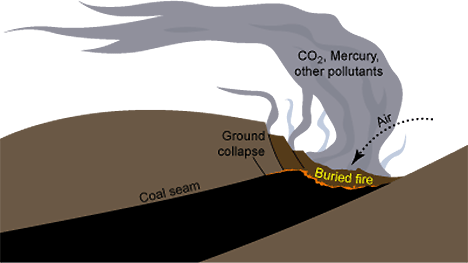
\includegraphics[width = 0.70\textwidth]{undergroundfire.png}
    \caption{Underground coal fire. Schematic showing subsidence and pollution that occurs with underground coal fires. }
    \label{fig:undergroundfire}
\end{figure}


Typically when fossil fuels are studied within the realm of environmental science, we focus on how relying on them for energy contributes to green house gases. In this chapter, we are going to delve into other ways in which fossil fuels affect the environment. By focusing on the extraction processes of different types of fuels, we will discover the ways in which surrounding ecosystems are directly affected by mining through land subsidence and ground water pollution. We will focus on China, as this is the largest fossil fuel producer and user in all of Asia. 


% \section{Underground Coal Fires in China} \cite{stracher2004coal}
%   \1 Cracks induced by subsidence measuring up to ``several kilometers long, tens of meters wide, and hundred of meters deep"
%       \2 Positive feedback loop- cracks increase oxygen circulation thereby promoting combustion 
%   \1 Economic loss estimated to be as high as \$25-250 million USD (Prakarsh)

% Citeint ``China: World�s Largest Energy Consumer and Greenhouse Gas Emitter"
%   \1 China 2012, coal is 66\% of energy, fossil fuels over 90\%
%   \1 China is estimated to contain over 90 billion tonnes of coal reserves. In 2016, the country produced 2.62 billion tonnes of coal. CITE(world energy council)






%%%%%%%%%%%%%%%%%%%%%%%%%%%%%
%What are fossil fuels
%%%%%%%%%%%%%%%%%%%%%%%%%%%%%

\section{Fossil Fuel Formation}

Before we can examine the ways in which fossil fuels are extracted, it is important that we understand what fossil fuels are, how they were formed, and when this all started.

\textbf{Fossil fuels} are hydrocarbons, meaning they are composed of hydrogen and carbon. This term typically includes coal, crude oil, and natural gas which all started to form millions of years ago from plant and animal remains. A combination of extremely high temperatures, high pressures, and millions of years allowed these organisms to be transformed into fossil fuels. 

\subsection{Coal Formation}

\subsubsection{Timeline}

The most significant coal formations stem from trees, ferns, and other plants that were growing during the Carboniferous ``coal-bearing" Period 290--360 million years ago. A combination of environmental factors, such as the evolution of large woody trees, allowed for coal deposits to begin to form during this time period. Lesser formations of coal continued through the Permian and Mesozoic Eras, 290--250 and 250--65 million years ago, respectively. Coal deposits that are less than 65 million years in age typically yield low quality coal, as they have not have enough time to fully transform into high-grade coal. 



\subsubsection{Process}


The first trees evolved around 360 million years ago at the beginning of the Carboniferous period. These ancient trees are the basis for our coal.  Coal formation begins with thousands of years of plant accumulation. This process starts with plants in wetland environments dying and beginning to decompose. This plant matter is then buried beneath new layers of plants which later die and add to the layers of organic matter beneath them. The resulting partially decomposed plant matter is known as \textbf{peat}. In tropical climates, the rate of peat accumulation is estimated to be about 2 meters every century. 

%%%%%%%%% Figure out a visual thingy %%%%%%%%% 
\emph{imagine a nifty graphic probably with a flow-chart vibe, showing the different levels in the coal formation process and the corresponding increasing carbon concentrations}
%%%%%%%%%%%%%%%%%%%%%%%%%%%%%%%%%%%%%%%%%%%%%%

As peat transforms to coal, it is further compacted to be about one-tenth of its original depth. As peat is increasingly buried, the resulting pressure transforms it into \textbf{lignite} which is low quality coal. When comparing the appearance of peat and lignite, we would find peat to contain some undecomposed plant material which lignite lacks. Additionally, lignite forms distinct geological layers. \cite{Xie2015}

The pressure and temperature continue to increase, allowing the low quality coal to progress to an intermediary sub-bituminous coal and then \textbf{bituminous coal}, the most widely spread type of coal.

Finally, with increasing pressure and a few more million years the high-grade coal, known as \textbf{anthracite}, is formed. The different types of coal contain varying concentrations of carbon: anthracite has the highest concentration which ranges from 86--98\% carbon, while lignite contains about 65--70\% carbon. \cite{Xie2015}


\subsection{Petroleum and Natural Gas Formation}

In a comparable manner to coal, petroleum and natural gas are formed over long periods of time as organic materials are compressed and heated. We previously saw that coal is formed from decaying terrestrial plants; in contrast, petroleum and natural gas originate from marine organisms, primarily zooplankton.

\begin{figure}[ht]
\centering
    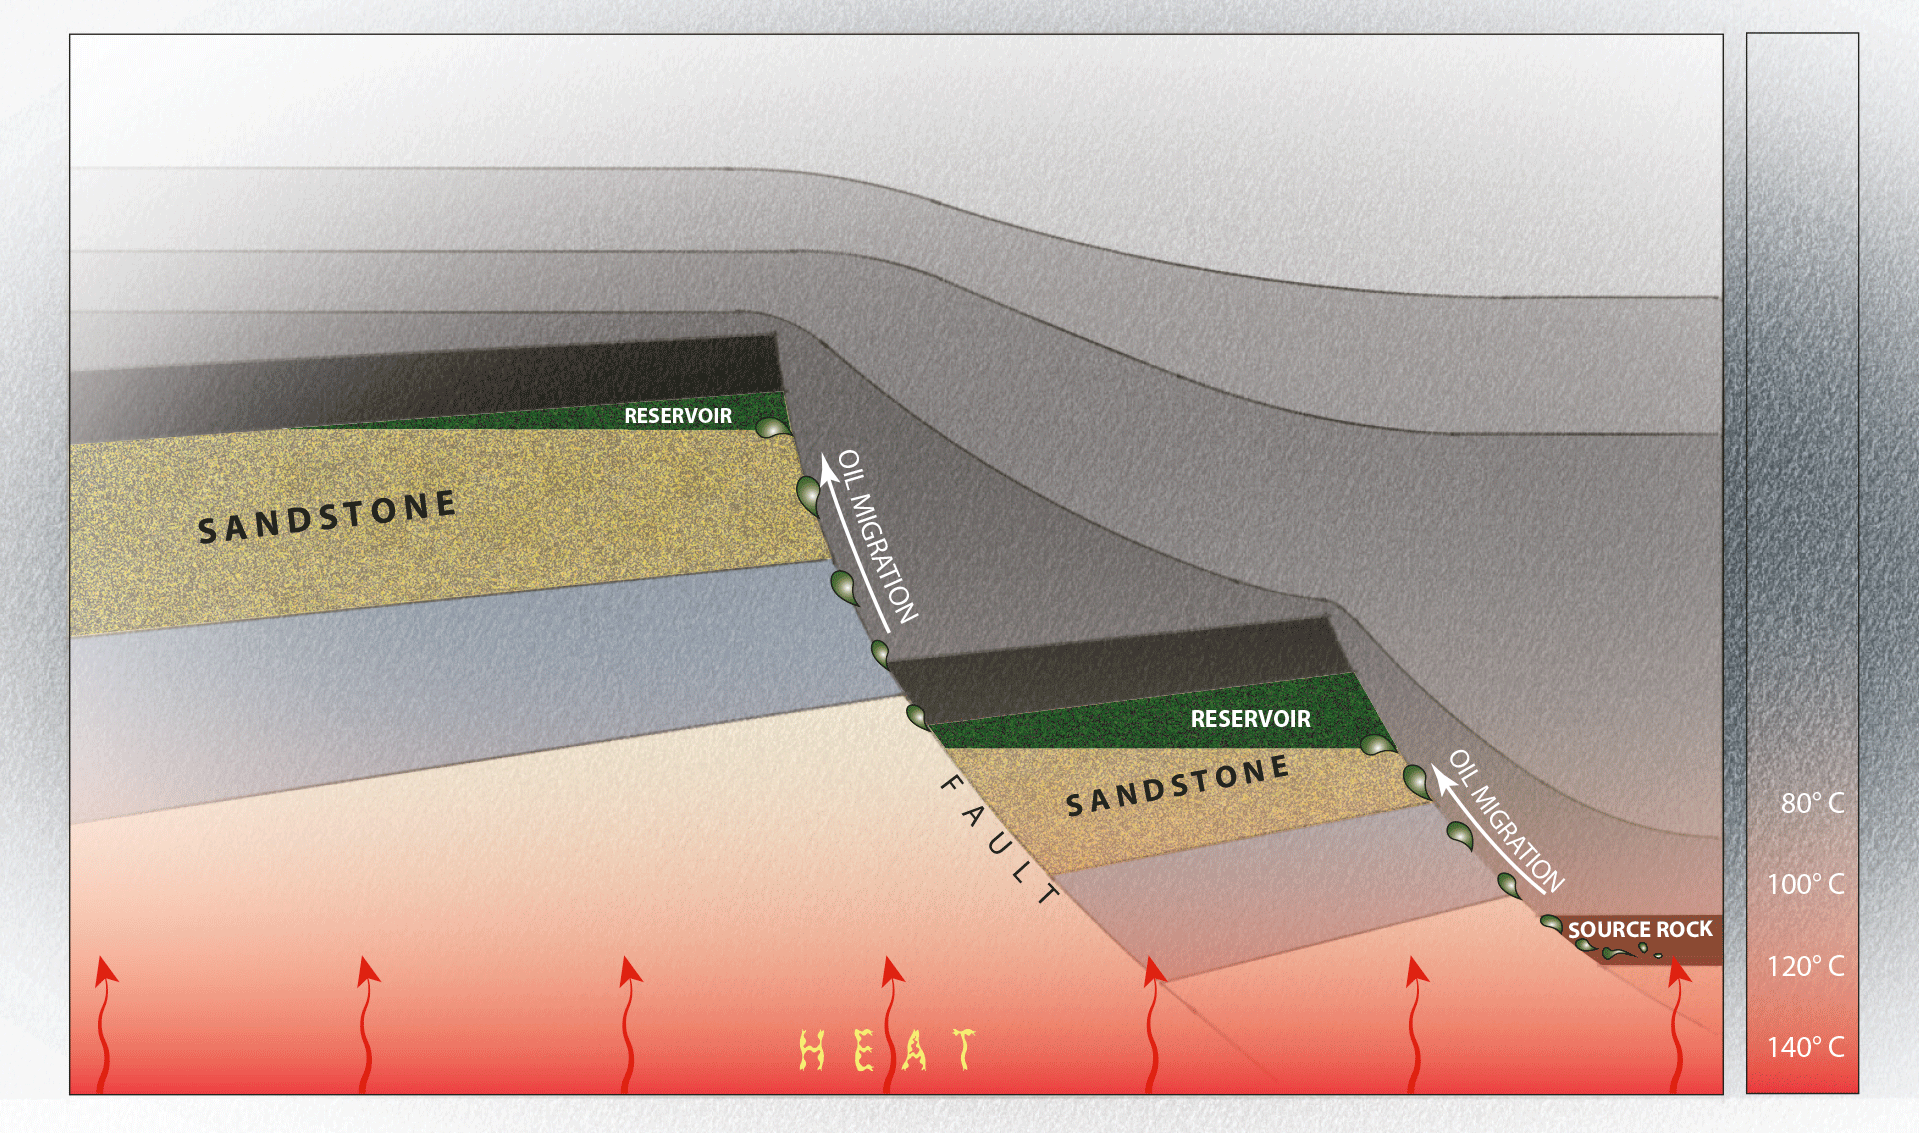
\includegraphics[width = 1\textwidth]{petroform.png}
    \caption{Formation of oil and gas reservoirs. Source: The Norwegian Petroleum Directorate }
    \label{fig:petroform}
\end{figure}


\emph{comparable to the coal stuff but more of an ocean vibe}
\subsubsection{Timeline}
\subsubsection{Process}

As the phytoplankton died, they sank to the seafloor and accumulated in the oxygen-free environment as sediment deposited on top of them. Over time, they 






%%%%%%%%%%%%%%%%%%%%%%%%%%%%%
%The fun stuff we've all been waiting for
%%%%%%%%%%%%%%%%%%%%%%%%%%%%%


\section{Methods of Coal Extraction}


Coal reserves are found throughout China, with recoverable reserves estimated at 324.1 billion tons 
%CITE WEITONG FROM JI. 
Figure~\ref{fig:coallocation} shows where these coal reserves are located throughout the country. The vast majority of this coal is not accessible via surface mining; in fact, only about 5--7 percent can be secured with this method. As of 2010, China was producing coal at a rate of 2.24 billion tons per year, of which surface mining accounted for about 9 percent. 


\begin{figure}[ht]
\centering
    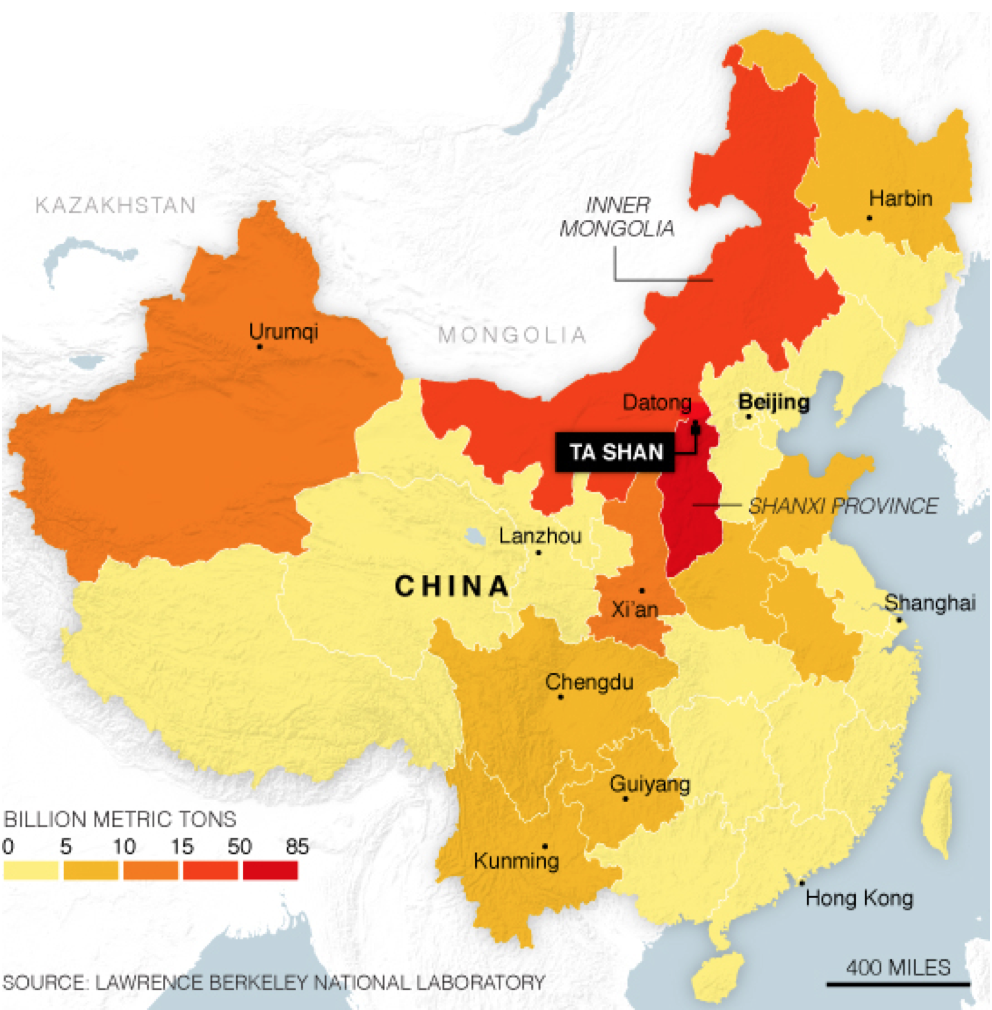
\includegraphics[width = 0.70\textwidth]{coallocation.png}
    \caption{Map of China's technically recoverable coal reserves by province. }
    \label{fig:coallocation}
\end{figure}

\subsection{Surface Coal Mining}
Threre are three distinct surface mining methods that are presently emplyed in China: open pit mining, area type mining, and contour mining. 

\subsubsection{Openpit Mining}


\begin{figure}[ht]
\centering
    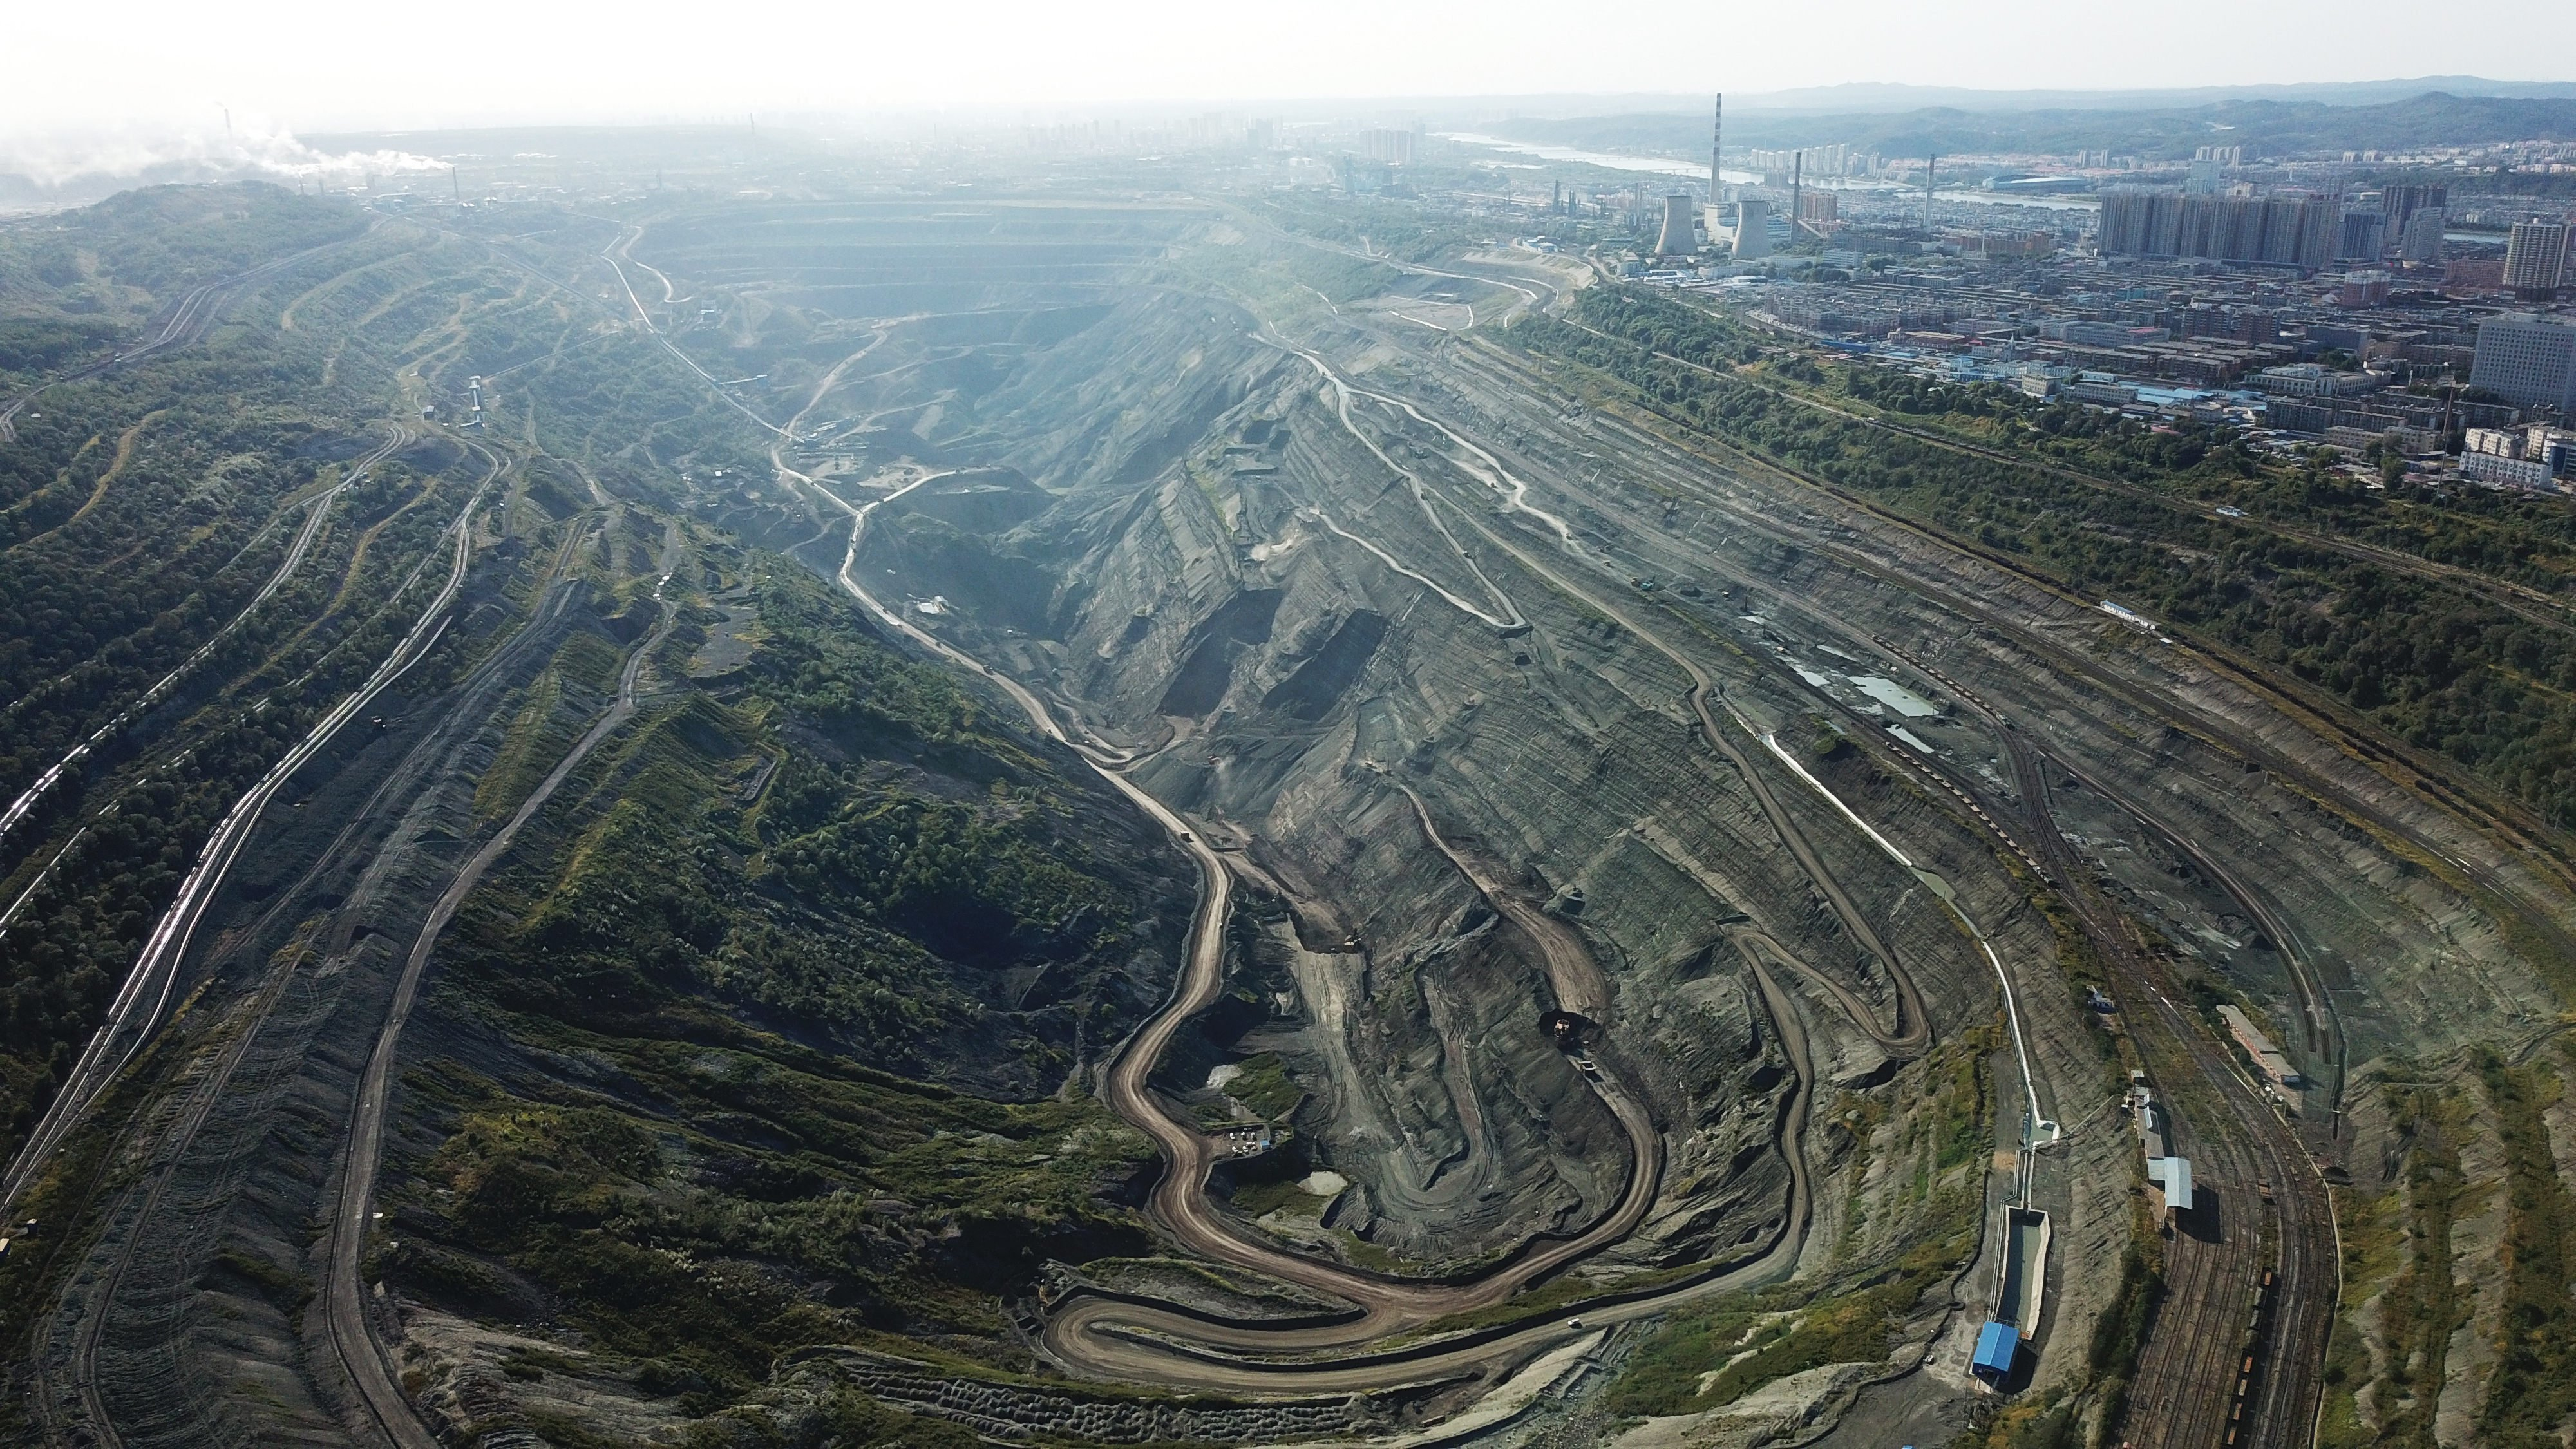
\includegraphics[width = 1.0\textwidth]{openpit.jpg}
    \caption{An open-pit coal mine, located in Fushun, in northeast China's Liaoning province. Image from Yan Bo of Zuma Press. }
    \label{fig:openpit}
\end{figure}

\subsubsection{Area Type Mining}

Area type mining is commonly employed in surface coal mines established after 1980 in China. 

In China, area type mining is characterized by the removal of coal seams ranging in thickness from 6 to 30 meters, with some being over 100 meters in thickness. 

\subsubsection{Contour Mining}


\cite{ji2012surface}
\subsection{Underground Coal Mining}


\subsubsection{ The Environmental Effects}
Coal mining does simply occur in uninhabited areas. The effects of subsidence are apparent in Da Antou, located in Shanxi province about 650 kilometers southwest of Beijing. This small village sits atop a mountain that is littered with underground coal mines. In 2007 the majority of the 200 houses in Da Antou were cracked, and more than a dozen have been declared unfit to be inhabited since 2005. Chen Xiao'e, a former resident of Da Antou, describes how her windows started to shatter before cracks appeared, several centimeters in width, in the walls of her three-year-old brick home. Finally the floor buckled and the house became entirely unsafe to live in. 










\subsection{Oil and Natural Gas}
\subsubsection{Drilling}
\subsubsection{Hydraulic fracturing (fracking)} 

Hydraulic fracturing, known more commonly as \textbf{fracking}, is an extraction method used to remove gas and oil from within impermeable shale rock. 

This method requires vertically drilling downward for about 2 km before turning to drill horizontally for as far as 3 km.  The fracking process itself is based in expelling fracking fluid, known as \textbf{slickwater}, at high pressures through small perforations in the horizontal pipe. The slickwater, composed of water, sand, and an assortment of additives, is forced out of the horizontal pipe at pressures above 600 atm creating microfractures for up to 50 m in the surrounding rock.

There are a number of environmental concerns surrounding fracking. 
\begin{itemize}
\item Water usage 

The fracking process requires extremely large volumes of water. INSERT NUMBER. Sourcing this much water can put a stress on surrounding surface and ground water reserves, particularly in desert regions such as INSERT LOCATION.
\item Water contamination 

The flowback liquid from fracking contains the original additives and may also contain heavy metals, radioactive material, and other toxins. Poorly constructed wells or other means of spilling this liquid could contaminate surrounding surface and ground water sources. 

\item Subsidence

As with other forms of fossil fuel extraction, removing and altering material from below ground tends to cause subsidence.

\item Methane

\end{itemize}



\section{Fossil Fuels and Asia}

\subsection{Fossil fuel production by country}


%%%%%%%%%%%%%%%%%%%%%%%%%%%%%
%The Economics, my main focus
%%%%%%%%%%%%%%%%%%%%%%%%%%%%%
\section{So why Fossil Fuels?}

\emph{The goal of this section is to show that while there are serious environmental/health effects associated with fossil fuels, we can't simply stop using them. I'll show that China, while incredibly dependent on coal, is actually one of the most efficient countries at processing coal. }

Let's now take a step back and briefly examine the economic and political reasons why countries like China are so dependent on fossil fuels and in particular, coal.  

While China is incredibly dependent on coal, its coal-fired power plants are significantly more efficient that those in the United States. In this context, efficiency refers to the amount of coal consumed per unit of power produced, and is thus related to gas emissions. 

Rapid growth, etc, etc, etc, relatively cheap option, reserves, etc